% Appendix A
\g
\chapter{Παράρτημα Κεφαλαίου 2} % Main appendix title

\label{AppendixB} % For referencing this appendix elsewhere, use \ref{AppendixA}

\section{Αναλυτική έκφραση προοπτικής προβολής}
\label{appendix:extensive_projection}

Στην πραγματικότητα παρεμβάλλονται κι άλλα φαινόμενα που χρήζουν μοντελοποίησης, ώστε η συνάρτηση $f_{pr}$ να είναι ακριβής. Μια πιο πλήρης περιγραφή της αποδίδεται από την παρακάτω σχέση: \cite{ma2012invitation}

\[ Z\begin{bmatrix}x \\ y \\ 1\end{bmatrix} = 
\begin{bmatrix}
\alpha & -\alpha\cot\theta & s_x & 0\\
0 & \frac{\beta}{\sin\theta} & s_y & 0\\
0 & 0 & 1 & 0 
\end{bmatrix} * 
\begin{bmatrix}
X \\ Y \\ Z \\ 1
\end{bmatrix}  \]

όπου:

\begin{itemize}
	\item $f$, η εστιακή απόσταση της κάμερας ($cm$)
	\item $k$, αναλογία $\frac{pixels}{cm}$ κατά τον άξονα $xx'$
	\item $l$, αναλογία $\frac{pixels}{cm}$ κατά τον άξονα $yy'$\footnote{η αναλογία είναι συνήθως διαφορετική κατά τους δύο άξονες, καθώς τα \e pixels \g είναι παραλληλόγραμμα}
	\item $ \alpha = k*f $, η εστιακή απόσταση εκφρασμένη σε μονάδες οριζόντιας πλευράς \e pixel \g
	\item $ \beta = l*f $, η εστιακή απόσταση εκφρασμένη σε μονάδες κάθετης πλευράς \e pixel \g
	\item $ [s_x,s_y]^T$,  μετατόπιση του κέντρου της εικόνας από το οπτικό κέντρο στο πάνω αριστερό άκρο ($pixel$)
	\item $ \theta $, απόκλιση της γωνίας των αξόνων της κάμερας από την τέλεια καθετότητα των $90^{\circ}$ μοιρών ($rad$)
 \end{itemize}
 
Το παραπάνω μοντέλο αγνοεί το φαινόμενο της ακτινικής παραμόρφωσης (\e radial distortion\g). Η ακτινική παραμόρφωση, όπως και η απόκλιση της γωνίας των αξόνων της κάμερας, δημιουργούν αποκλίσεις που διορθώνονται με κατάλληλη επεξεργασία \e(camera calibration). \g Προκειμένου να δώσουμε έμφαση στα ζητήματα της στερεοσκοπικής γεωμετρίας, οι μαθηματικές σχέσεις που χρησιμοποιούμε δεν περιλαμβάνουν αυτά τα φαινόμενα.


\section{Αναλυτική έκφραση ευθείας}
\label{appendix:extensive_projection_line}

Αν έχουμε μοντελοποιήσει την προοπτική προβολή μέσω της έκφρασης του κεφαλαίου \ref{appendix:extensive_projection}, η ευθεία που ενώνει το οπτικό κέντρο $O$ της κάμερας με το σημείο $\mathbf{p}$ δίνεται από την παρακάτω πιο αναλυτική διανυσματική έκφραση:

$$ (X,Y,Z) = t\cdot \left ( \dfrac{x-s_x}{a} + \dfrac{\cot \theta \sin \theta y s_y}{\beta} , \dfrac{(y-s_y) \sin \theta}{\beta} , 1\right),  t \in [f,+\infty) $$

\section{Απόδειξη στερεοσκοπικού περιορισμού}
\label{appendix:epipolar_constraint_proof}

Υπόθεση:

\begin{enumerate}
	\item Ως σύστημα αναφοράς έχουμε ορίσει το σύστημα συντεταγμένων της αριστερής λήψης.
	\item Γνωρίζουμε τον \e affine \g μετασχηματισμό $g = (R,T)$ που προσδιορίζει την θέση και τον προσανατολισμό της δεξιάς λήψης.
	\item Συμβολίζουμε με $\mathbf{p_1},\mathbf{p_2}$ τις προβολές του \textbf{ίδιου} \e 3D \g σημείου στο σύστημα συντεταγμένων της αριστερής και δεξιάς λήψης αντίστοιχα
\end{enumerate}

Τότε τα δύο αντίστοιχα σημεία τηρούν την σχέση: $$\mathbf{p_2}^{T} E \mathbf{p_1} = 0, \text{όπου} \: E = [T]R$$ Ως $[T]$ συμβολίζουμε τον πίνακα εξωτερικού γινομένου του διανύσματος $T$. 

Ο πίνακας $E$ ονομάζεται \e essential matrix. \g 

Για δεδομένο σημείο $\mathbf{p_1}$ αναζητούμε το "αντίστοιχο σημείο" $\mathbf{p_2}$. Η απόδειξη ισχύει και για το αντίστροφο:

\begin{equation}
\begin{gathered}
	\mathbf{P_2}  = R\mathbf{P_1} + T \Leftrightarrow \\
	f \cdot \begin{bmatrix} \sfrac{X_2}{Z_2} \\ \sfrac{Y_2}{Z_2} \\ 1 \end{bmatrix} = R \cdot f
	\begin{bmatrix} \sfrac{X_1}{Z_1} \\ \sfrac{Y_1}{Z_1} \\ 1 \end{bmatrix} + T \xRightarrow{[T] \cdot} \\
	f \cdot [T] \begin{bmatrix} \sfrac{X_2}{Z_2} \\ \sfrac{Y_2}{Z_2} \\ 1 \end{bmatrix} = f \cdot[T] \cdot R
	\begin{bmatrix} \sfrac{X_1}{Z_1} \\ \sfrac{Y_1}{Z_1} \\ 1 \end{bmatrix} + [T]T \xLeftrightarrow{[T]T=0} \\
	[T] \begin{bmatrix} \sfrac{X_2}{Z_2} \\ \sfrac{Y_2}{Z_2} \\ 1 \end{bmatrix} = [T] \cdot R
	\begin{bmatrix} \sfrac{X_1}{Z_1} \\ \sfrac{Y_1}{Z_1} \\ 1 \end{bmatrix} \xRightarrow{\mathbf{p_2^T}\cdot} \\
	\begin{bmatrix} \sfrac{X_2}{Z_2} & \sfrac{Y_2}{Z_2} & 1 \end{bmatrix} [T] \begin{bmatrix} \sfrac{X_2}{Z_2} \\ \sfrac{Y_2}{Z_2} \\ 1 \end{bmatrix} = \begin{bmatrix} \sfrac{X_2}{Z_2} & \sfrac{Y_2}{Z_2} & 1 \end{bmatrix} [T] \cdot R
	\begin{bmatrix} \sfrac{X_1}{Z_1} \\ \sfrac{Y_1}{Z_1} \\ 1 \end{bmatrix} \xLeftrightarrow{\mathbf{p_2} \perp T \times\mathbf{p_2}} \\	
	0 = \begin{bmatrix} \sfrac{X_2}{Z_2} & \sfrac{Y_2}{Z_2} & 1 \end{bmatrix} [T] \cdot R
	\begin{bmatrix} \sfrac{X_1}{Z_1} \\ \sfrac{Y_1}{Z_1} \\ 1 \end{bmatrix}  \Leftrightarrow \\
	\mathbf{p_2}^{T} [T_x] R \mathbf{p_1} = 0 \xRightarrow{E=[T] R} \\
	\mathbf{p_2}^{T} E \mathbf{p_1} = 0
\end{gathered}
\end{equation}


\section{Λήψη εικόνας από στερεοσκοπική διάταξη}
\label{appendix:stereo_constraint_from_stereo_rig}

Στη στερεοσκοπική διάταξη, η θέση της δεξιάς λήψης προκύπτει από αυτή της αριστερής, με μετατόπισης μόνο κατά τον άξονα $xx'$ και χωρίς καμία περιστροφή. \ref{fig:stereo_rig} Ισχύουν επομένως οι εξής περιορισμοί: 

\begin{gather}
	g_{stereo} = \left( R=I,T = \begin{bmatrix}
		b \\ 0 \\ 0
	\end{bmatrix} \right)
	\\
	E_{stereo} = 
	\begin{bmatrix}
		0 & 0 & 0 \\ 0 & 0 & -b \\ 0 & b & 0
	\end{bmatrix}
	\begin{bmatrix}
		1 & 0 & 0 \\ 0 & 1 & 0 \\ 0 & 0 & 1
	\end{bmatrix} =
	\begin{bmatrix}
		0 & 0 & 0 \\ 0 & 0 & -b \\ 0 & b & 0
	\end{bmatrix}
\end{gather}


\begin{equation}
	\setlength{\jot}{10pt}
	\begin{gathered}
		p_1^{T}Ep_2 = 0 \Leftrightarrow 
		\\
		\begin{bmatrix}
		x_1 & y_1 & 1
		\end{bmatrix}
		\begin{bmatrix}
		0 & 0 & 0 \\ 0 & 0 & -b \\ 0 & b & 0
		\end{bmatrix}\begin{bmatrix}
		1 & 0 & 0 \\ 0 & 1 & 0 \\ 0 & 0 & 1
		\end{bmatrix}
		\begin{bmatrix}
		x_2 \\ y_2 \\ 0
		\end{bmatrix} = 0 \Rightarrow
		\\
		\begin{bmatrix}
		x_1 & y_1 & 1
		\end{bmatrix}
		\begin{bmatrix}
		0 \\ -b \\ by_2
		\end{bmatrix} = 0 \Rightarrow
		\\
		-by_1 + by_2 = 0 \Rightarrow
		\\
		y_1 = y_2
	\end{gathered} \label{eq:stereo_constraint}
\end{equation}

Ο περιορισμός \ref{eq:stereo_constraint} ονομάζεται στερεοσκοπικός περιορισμός \e (stereo constraint) \g κι αποδεικνύει ότι η στερεοσκοπική διάταξη ικανοποιεί με φυσικό τρόπο τον ορισμό της στερεοσκοπικής όρασης. 

\section{Ευθυγράμμιση \texorpdfstring{\e (Rectification) \g}{TEXT}}
\label{appendix:stereo_constraint_from_rectification}

Δεν είναι μονόδρομος η χρήση στερεοσκοπικής διάταξης για να επιτευχθεί ο στερεοσκοπικός περιορισμός. Αντιθέτως, μπορεί να επιβληθεί μετά την λήψη των εικόνων με κατάλληλη επεξεργασία. Αν γνωρίζουμε τον \e affine \g μετασχηματισμό $g = (R,T)$, η μετατροπή του τυχαίου ζεύγους εικόνων σε στερεοσκοπικό είναι άμεση\citep{faugeras1993three}. Αν επίσης αγνοούμε πλήρως την σχετική θέση των δύο λήψεων, μπορούμε πρώτα να υπολογίσουμε τον πίνακα $E = [T_x]R \in \mathbb{R}^{3\times3}$ μέσω κάποιας κατάλληλης τεχνικής (π.χ. αλγόριθμος 8 σημείων) κι ακολούθως να μετατρέψουμε το ζεύγος σε στερεοσκοπικό. Αμφότερα τα σενάρια είναι αντιμετωπίσιμα, με το πρώτο να έχει μεγαλύτερη ακρίβεια σε σχέση με το δεύτερο που συσσωρεύει κάποιο σφάλμα λόγω του εισαγωγικού βήματος του υπολογισμού του πίνακα $E$.

Η αναλυτική μεθοδολογία επίλυσης του προβλήματος ευθυγράμμισης (όπως και της εύρεσης του πίνακα $E$ όταν είναι αναγκαίο) ξεφεύγει των σκοπών της συγκεκριμένης εργασίας. Παρακάτω δίνεται μια σύντομη περιγραφή των βημάτων της ευθυγράμμισης για την εποπτική κατανόηση της μεθοδολογίας: \citep{trucco1998introductory}

Υποθέτουμε ότι γνωρίζουμε \e affine \g μετασχηματισμό $g = (R,T)$. Τότε:

\begin{itemize}
	\item Περιστρέφουμε την αριστερή λήψη ώστε η ευθεία βάσης (ευθεία που συνδέει το οπτικό κέντρο των δύο λήψεων) με το επίπεδο που ορίζει το πέτασμα της αριστερής κάμερας να γίνουν παράλληλα. Ο πίνακας που υλοποιεί αυτήν την περιστροφή ονομάζεται $R_{rect} \in \mathbb{R}^{3\times 3} : \parallel R_{rect}\parallel = 1$.
	\item Η αντίστοιχη πίνακας για την δεξιά λήψη είναι ο $R_r = RR_{rect} \in \mathbb{R}^{3\times 3}$
	\item Για κάθε σημείο της αριστερής λήψης $\mathbf{p}_L \in I^L$ υπολογίζουμε:
	$$R_{rect}\mathbf{p}_L = [x',y',z'] \Rightarrow$$
	$$\Rightarrow \mathbf{p}_{L}^{'} = [f\cdot \dfrac{x'}{z'},f\cdot \dfrac{y'}{z'},f]$$
	\item Αντίστοιχα για την δεξιά λήψη, υπολογίζουμε τα σημεία $\mathbf{p}_{R}^{'}$ με χρήση του $R_r$ αντί του $R_{rect}$
\end{itemize}

Όσα περιγράφηκαν παραπάνω σε επίπεδο σημείου $\mathbf{p}$ μπορούν να εφαρμοστούν συνολικά σε όλα τα σημεία του πετάσματος κι έτσι επιτυγχάνεται η δημιουργία ενός ζεύγους εικόνων που τηρεί τον στερεοσκοπικό περιορισμό. Πρέπει να παρατηρήσουμε ότι ενώ οι προ ευθυγράμμισης τιμές των σημείων είναι ακέραιοι αριθμοί (θέσεις \e pixel) \g οι επιστρεφόμενες τιμές είναι πραγματικοί αριθμοί. Επομένως, πρέπει να εφαρμοστεί ένα βήμα παρεμβολής τιμών σε ορθογώνιο χωρίο για τον υπολογισμό της τελικής ευθυγραμμισμένης εικόνας.

Η ευθυγράμμιση γενικεύει την αξία του προβλήματος της στερεοσκοπικής όρασης, αυξάνοντας το πεδίο εφαρμογής του από το στενό πλαίσιο των στερεοσκοπικών διατάξεων σε κάθε ζεύγος εικόνων, οποιασδήποτε γεωμετρίας. 

\begin{figure}
	\centering
	\begin{subfigure}{.8\textwidth}
		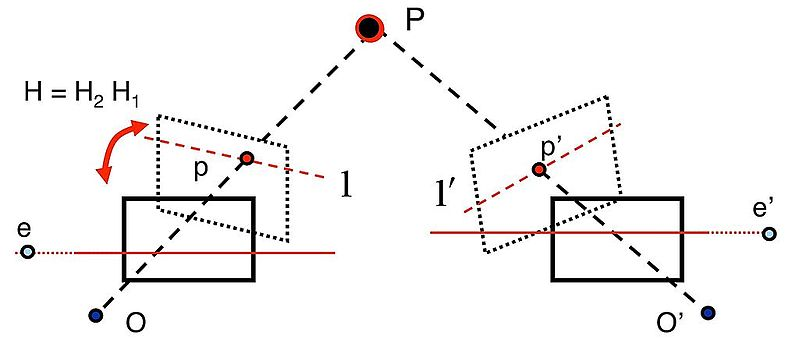
\includegraphics[width=\textwidth]{rectification_geometry.jpg}
		\caption{Γεωμετρική αποτύπωση της ευθυγράμμισης ενός ζεύγους εικόνων}
	\end{subfigure}
	
	\begin{subfigure}{.25\textwidth}
		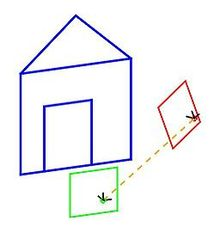
\includegraphics[width=\textwidth]{rectification1.jpg}
		\caption{Το αρχικό σχήμα που φωτογραφίζουν οι δύο κάμερες.}
	\end{subfigure}
	\begin{subfigure}{.74\textwidth}
		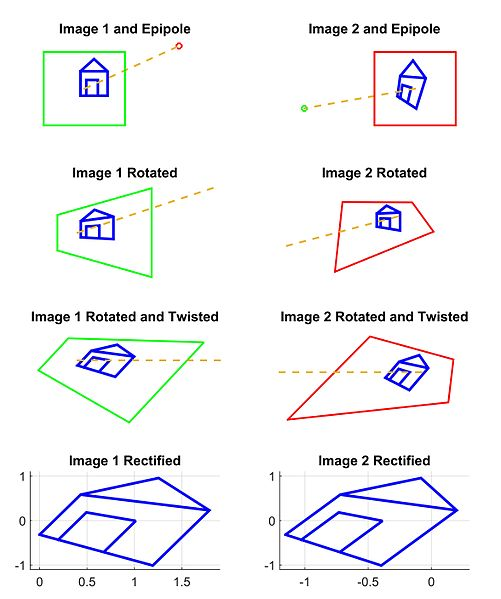
\includegraphics[width=\textwidth]{rectification2.jpg}
	\end{subfigure}
	\caption{Αναλυτική παρουσίαση των μετασχηματισμών που ευθυγραμμίζουν το αρχικό ζεύγος εικόνων. Πηγή: \citep{WikipediaRectification}}
	\label{fig:rectification_geometry}
\end{figure}

\begin{figure}
	\centering
	\begin{subfigure}{.49\textwidth}
		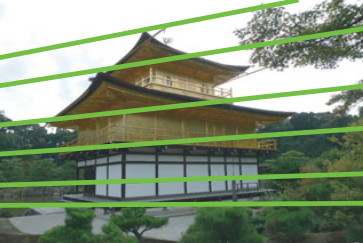
\includegraphics[width=\textwidth, height = 0.7\textwidth]{rectified_before_l.png}
	\end{subfigure}
	\begin{subfigure}{.49\textwidth}
		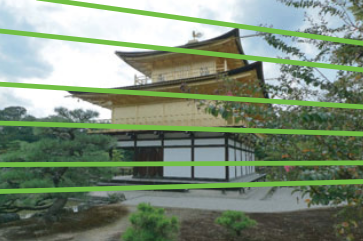
\includegraphics[width=\textwidth, height = 0.7\textwidth]{rectified_before_r.png}
	\end{subfigure}
	
	\begin{subfigure}{.49\textwidth}
		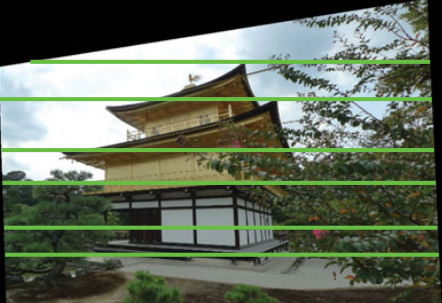
\includegraphics[width=\textwidth, height = 0.7\textwidth]{rectified_after_l.png}
	\end{subfigure}
	\begin{subfigure}{.49\textwidth}
		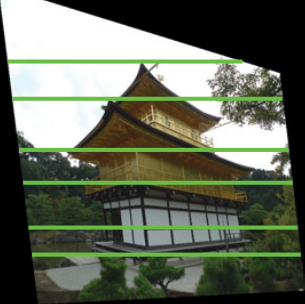
\includegraphics[width=\textwidth, height = 0.7\textwidth]{rectified_after_r.png}
	\end{subfigure}
	\caption{Παράδειγμα ευθυγράμμισης από το βιβλίο \e Computer vision for visual effects. \g \citep{radke2013computer}. Επάνω: ζεύγος εικόνων τυχαίας γεωμετρίας. Κάτω: ζεύγος εικόνων που τηρεί τον στερεοσκοπικό περιορισμό, μετά από ευθυγράμμιση.}
	\label{fig:rectification_example}
\end{figure}

\section{Επαναληπτική εφαρμογή φίλτρου μέσου όρου κατά την άθροιση κόστους σε ορθογώνια περιοχή}
\label{appendix:mean2gaussian}

Η επαναληπτική εφαρμογή του φίλτρου μέσου όρου φαίνεται παρακάτω:

\begin{align*} 
C_{agg}^{0} &= C_{init} \\
C_{agg}^{k}(d,x,y) &= C_{agg}^{k-1}(x,y,d) \ast h(x,y)
\end{align*}

που ισοδυναμεί με συνέλιξη του αρχικού πίνακα κόστους με το φίλτρο: \e
\begin{gather*} 
h_1 = \underbrace{h(x,y) \ldots \ast h(x,y)}_{\text{k times}} \\ 
C_{agg}^{n}(d,x,y) = C_{init}(x,y,d) \ast h_1
\end{gather*}
\g

Παρατηρούμε ότι η επαναληπτική συνέλιξη του φίλτρου με τον εαυτό του, αυξάνει σε κάθε βήμα τις διαστάσεις του. Πιο συγκεκριμένα, έστω παράθυρο $h$ με αρχικές διαστάσεις $m \times n$, η επαναληπτική εφαρμογή του $k$ φορές στον αρχικό πίνακα κόστους ισοδυναμεί, με συνέλιξή του με ένα φίλτρο διαστάσεων
\begin{gather*} 
m_1 = m + (m-1)*(k-1) \\ 
n_1 = n + (n-1)*(k-1)
\end{gather*}

Η γραμμική αύξηση των διαστάσεων του ισοδύναμου φίλτρου κατά την αναδρομική άθροιση κόστους γειτονιάς φέρει τις ίδιες αδυναμίες και πλεονεκτήματα με την εξ' αρχής επιλογή μεγάλης περιοχής υποστήριξης. Υπάρχει βέβαια ποιοτική διαφορά μεταξύ τους καθώς η επαναληπτική συνέλιξη με τον εαυτό του τείνει να το μετατρέψει σε γκαουσιανό φίλτρο \e(gaussian filter)\g, όπως παρατηρούμε στο σχήμα \ref{fig:mean_filter_iterations} Για παράδειγμα εάν εφαρμόσουμε ένα απλό $3 \times 3$ φίλτρο 2 και 3 και 4 φορές αντίστοιχα θα είναι σαν να είχαμε κάνει αρχική συνέλιξη με τα φίλτρα:

\[
h =
\begin{bmatrix}
  1 & 1 & 1\\
  1 & 1 & 1\\
  1 & 1 & 1\\
\end{bmatrix}
\]

\[
h_1 = \dfrac{1}{9} 
\begin{bmatrix}
  1 & 2 & 3 & 2 & 1\\
  2 & 4 & 6 & 4 & 2\\
  3 & 6 & 9 & 6 & 3\\
  2 & 4 & 6 & 4 & 2\\
  1 & 2 & 3 & 2 & 1\\
\end{bmatrix}
\]

\[
h_2 = \dfrac{1}{9^2} 
\begin{bmatrix}
  1 & 3 & 6 & 7 & 6 & 3 & 1\\
  3 & 9 & 18 & 21 & 18 & 9 & 3\\
  6 & 18 & 36 & 42 & 36 & 18 & 6\\
  7 & 21 & 42 & 49 & 42 & 21 & 7\\
  6 & 18 & 36 & 42 & 36 & 18 & 6\\
  3 & 9 & 18 & 21 & 18 & 9 & 3\\
  1 & 3 & 6 & 7 & 6 & 3 & 1\\
 \end{bmatrix}
\]

\[
h_3 = \dfrac{1}{9^3} 
\begin{bmatrix}
  1 & 4 & 10 & 16 & 19 & 16 & 10 & 4 & 1\\
  4 & 16 & 40 & 64 & 76 & 64 & 40 & 16 & 4\\
  10 & 40 & 100 & 160 & 190 & 160 & 100 & 40 & 10\\
  16 & 64 & 160 & 256 & 304 & 256 & 160 & 64 & 16\\
  19 & 76 & 190 & 304 & 361 & 304 & 190 & 76 & 19\\
  16 & 64 & 160 & 256 & 304 & 256 & 160 & 64 & 16\\
  10 & 40 & 100 & 160 & 190 & 160 & 100 & 40 & 10\\
  4 & 16 & 40 & 64 & 76 & 64 & 40 & 16 & 4\\
  1 & 4 & 10 & 16 & 19 & 16 & 10 & 4 & 1\\
\end{bmatrix}
\]

Η σταδιακή μετατροπή σε γκαουσιανό φίλτρο, πέρα από την αύξηση της περιοχής υποστήριξης, δίνει ιδιαίτερη βαρύτητα στα \e(pixels) \g κοντά στο \e(pixel) \g ενδιαφέροντος, αδιαφορώντας για το πιο απομακρυσμένα.

\begin{figure}
	\centering
	\begin{subfigure}{.6\textwidth}
		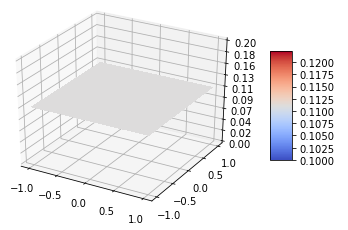
\includegraphics[width=\textwidth]{mean_iter1.png}
		\caption{επανάληψη 1}
	\end{subfigure}
	\begin{subfigure}{.6\textwidth}
		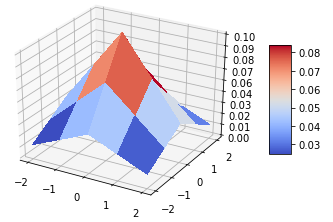
\includegraphics[width=\textwidth]{mean_iter2.png}
		\caption{επανάληψη 2}
	\end{subfigure}
	\begin{subfigure}{.6\textwidth}
		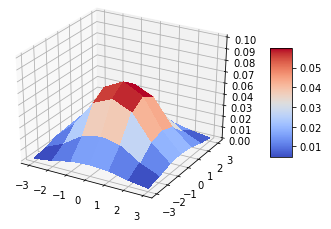
\includegraphics[width=\textwidth]{mean_iter3.png}
		\caption{επανάληψη 3}
		\label{fig:small_window}
	\end{subfigure}
		\begin{subfigure}{.6\textwidth}
		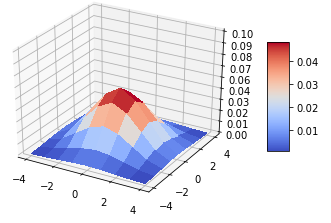
\includegraphics[width=\textwidth]{mean_iter4.png}
		\caption{επανάληψη 4}
		\label{fig:large_window}
	\end{subfigure}
	\caption{μεταβολή $3\times3$ φίλτρου μέσης τιμής κατά την συνέλιξη με τον εαυτό του}
	\label{fig:mean_filter_iterations}
\end{figure}
